\subsection{Glyph: \glyph{Or}}
\label{sec:af:or}

The glyph \glyph{or} is used to denote that any of the \glyph{ANs} linked as input is sufficient to influence the target activity.

\begin{glyphDescription}
 \glyphSboTerm SBO:0000174 ! or.
 \glyphIncoming One or more \glyph{logic arcs} (\sect{af:logicArc}).
 \glyphOutgoing  One \glyph{logic arc} (\sect{af:logicArc}) or one of the modulation arcs (\sect{af:arcs}).
 \glyphContainer An \glyph{or} operator is represented by a circular shape containing the word ``OR''.
The shape is linked to two ports, that are small arcs attached to the centres of opposite sides of the shape, as shown in \fig{af:or}.
The incoming \glyph{logic arcs} (\sect{af:logicArc}) are linked to the extremity of the leftmost or uppermost port, while the outgoing \glyph{logic arc} (\sect{af:logicArc}) or modulation arc (\sect{af:arcs}) is linked to the extremity of the rightmost or bottommost port.
 \glyphLabel None.
 \glyphAux None.
 \end{glyphDescription}

\begin{figure}[H]
  \centering
  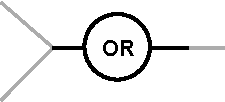
\includegraphics[scale = 1]{images/build/or.pdf}
  \caption{The \AF glyph for \glyph{or}. Only two inputs are represented, but more would be allowed.}
  \label{fig:af:or}
\end{figure}


\begin{figure}[H]
  \centering
  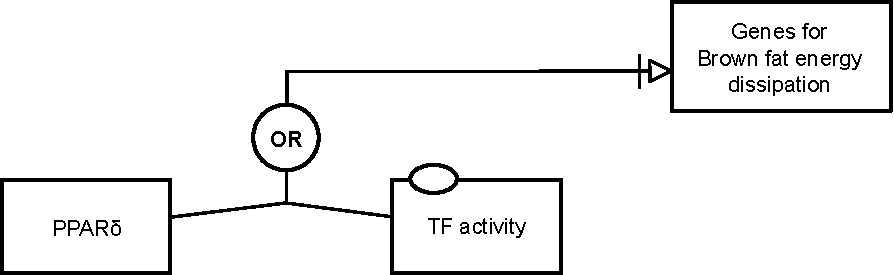
\includegraphics[scale = 0.8]{src/images/build/or_example.pdf}
  \caption{An example, taken from \fig{af:1}, of the \glyph{or} logic operator, where the activity from \glyph{"Genes for brown fat energy dissipation"} is stimulated by either the \glyph{PPAR delta} activity or an \glyph{unspecified transcription factor} activity.}
  \label{fig:af:ex-or}
\end{figure}
